\documentclass[11pt]{article}

\usepackage[margin=1in]{geometry}
\usepackage[T1]{fontenc}
\usepackage[utf8]{inputenc}
\usepackage{lmodern}
\usepackage{amsmath, amssymb, amsthm}
\usepackage{booktabs}
\usepackage{graphicx}
\usepackage{xcolor}
\usepackage{hyperref}
\usepackage{enumitem}
\usepackage{natbib}
\usepackage{setspace}
\usepackage{caption}
\usepackage{float}

\hypersetup{
  colorlinks=true,
  linkcolor=blue,
  citecolor=blue,
  urlcolor=blue
}

\setstretch{1.08}
\setlength{\parskip}{0.4em}
\setlength{\parindent}{0pt}
\raggedbottom

\title{From Noisy ETF Features to Low-Turnover Alpha:\\
Rolling-Universe Evidence from U.S. Equities}

\author{
  Jingze Fu \\
  UCLA \\
  \texttt{fujingze1019@g.ucla.edu}
  \and
  [Coauthor Name] \\
  UCLA \\
  \texttt{[coauthor email]}
}

\date{}

\begin{document}

\maketitle

\begin{abstract}
We study whether ETF-linked information can improve daily stock return forecasting in U.S. equities when performance is judged in economic rather than purely statistical terms. The empirical design combines rolling-window estimation, Ridge-based return prediction, and an explicit execution layer with holding-period and rebalance controls. The starting point is negative out-of-sample $R^2$: large raw ETF feature blocks perform poorly and do not reliably outperform a stock-only HAR baseline. The evidence instead indicates that ETF-linked information is most useful when it enters through small, stock-specific adjustments rather than as a large covariate block. On that basis, we construct three strategies: a consensus-majority ETF signal, a regime-dependent ETF refinement, and a conservative baseline-plus-top3-ETF blend. We evaluate them with AlphaMark and with separate transaction-cost sensitivity checks at 10, 20, and 50 basis points. The best gross AlphaMark slices reach Sharpe ratios around 0.5--0.6, and the strongest specifications remain competitive with an optimized baseline after cost adjustments. Overall, ETF information is not effective as a raw feature expansion, but it can become economically useful when incorporated through low-dimensional signal design and disciplined execution.

\end{abstract}

\section{Introduction}

Predicting daily stock returns is difficult because the signal-to-noise ratio is low and many seemingly informative covariates degrade out-of-sample performance once estimation error, instability, and turnover are taken into account. In this project, we study whether ETF-linked information can improve stock-level daily return forecasting in U.S. equities.

The original motivation was straightforward. A stock's own past returns may miss broader cross-asset information visible in sector and macro ETF movements. In practice, however, raw ETF expansion performs poorly out of sample and does not translate into convincing economic value. The relevant question is therefore not whether ETF information can replace the stock-only baseline, but whether it can improve that baseline when introduced through a more selective design.

Accordingly, the analysis emphasizes portfolio PnL, AlphaMark diagnostics, and transaction-cost stress tests rather than mean squared error or out-of-sample $R^2$ alone. Methodologically, we also replace a fixed long-horizon stock panel with a rolling-universe, window-sliced design that better matches the available data and reduces survivorship-style distortions. In spirit, the project is related to HAR-style forecasting and empirical asset pricing with machine learning \citep{corsi2009simple,gu2020empirical}, but the emphasis here is not on proposing a new generic estimator. The central issue is how ETF-linked information should be represented and traded.

The main empirical message is that raw ETF information is not effective as a standalone predictor, but the relatedness structure between stocks and ETFs still contains useful directional content. Once that information is summarized through stock-specific signals and combined with explicit holding-period and rebalance rules, it becomes economically relevant. The final strategies are therefore not ``ETF replaces baseline'' models, but ETF-conditioned extensions of a stock-only HAR baseline. Importantly, the appropriate benchmark is not the raw baseline alone, but an optimized baseline with similarly disciplined execution. The strongest ETF-conditioned strategies are best interpreted as competitive refinements to that benchmark rather than as universal replacements for it.

Our main contributions are the following:
\begin{enumerate}[leftmargin=1.4em]
  \item We implement a rolling-universe, window-sliced forecasting pipeline for U.S. equities with a 10-year training window and a 1-year test window, allowing model-specific eligibility and time-varying coverage.
  \item We show that direct raw ETF expansion performs poorly, while stock-specific ETF summaries remain useful when introduced through confirmation, adjustment, and regime-dependent rules.
  \item We evaluate the signals in economic rather than purely statistical terms, using AlphaMark, explicit turnover-based cost stress tests, and a normalized-dollar-volume diagnostic to study liquidity dependence.
\end{enumerate}

The rest of the report is organized as follows. Section~\ref{sec:data} describes the data and problem setup. Section~\ref{sec:methodology} presents the rolling-universe forecasting and execution framework. Section~\ref{sec:strategy} describes the final signal designs. Section~\ref{sec:results} reports the main economic results. Section~\ref{sec:discussion} discusses interpretation, novelty, and limitations.

\section{Related Work}
\label{sec:related}

This project is related to three strands of literature.

\subsection{Cross-Sectional Return Prediction}

The first strand studies cross-sectional return prediction using characteristics, factors, and statistical learning methods. Classic asset-pricing work emphasizes the difficulty of explaining and forecasting the cross section of expected returns \citep{fama1992cross}. More recent machine-learning work shows that flexible predictive models can extract useful information from large panels of return predictors, but also makes clear that overfitting, instability, and implementation concerns remain central \citep{gu2020empirical}. Our project belongs to this tradition, but differs in focus: rather than expanding the predictor set as much as possible, we study whether ETF-linked information is more useful when it is represented parsimoniously and evaluated in economic terms.

\subsection{Economically Linked Securities and Network Ideas}

The second strand studies return comovement and predictability across economically linked securities. Work such as \citet{cohen2008economic} shows that return information can propagate across linked firms, while network-based asset-pricing papers such as \citet{ahern2013network} highlight the role of relationship structure in the cross section. Our original motivation is closest to this line of thinking. However, the empirical outcome of the project is more nuanced than a simple network-success story. The ETF-based network intuition remains useful as a way to think about relatedness and peer structure, but the final strongest implementations come from low-dimensional ETF-conditioned correction signals rather than from the network term alone.

\subsection{Economic Significance, Trading Costs, and Implementation}

The third strand emphasizes that predictive signals should be judged by economic usefulness rather than by statistical fit alone. In practice, turnover, market impact, and trading costs can materially alter the ranking of otherwise attractive signals \citep{frazzini2018trading,novymarx2016taxonomy}. Our project is directly aligned with this perspective. The move from negative out-of-sample $R^2$ toward PnL, AlphaMark, and explicit execution constraints therefore reflects a change in the object of interest: not simply prediction accuracy, but whether a signal survives implementation frictions.

Relative to these literatures, our contribution is modest but distinct. We do not propose a new general-purpose estimator. Instead, we show that ETF-linked information, while ineffective as a large raw block, can still matter when converted into stock-specific low-dimensional signals and evaluated under a rolling-universe framework with explicit execution constraints.

\section{Data and Problem Setup}
\label{sec:data}

\subsection{Universe and Sample Window}

Our stock panel spans 1990-01-17 to 2023-12-29, while the ETF feature panel spans 1993-02-01 to 2023-12-29. The final evaluation window reported in this project is 2006-01-03 to 2023-12-29. We focus on this range for three reasons. First, it provides a sufficiently mature ETF feature history. Second, it supports the 10-year rolling training design while still delivering a long out-of-sample period. Third, it aligns cleanly with the final AlphaMark evaluation pipeline used in the project.

The unit of observation is a stock-day pair. For each day, we merge stock-level return and size information with the corresponding ETF return panel. The working panel is therefore a multi-asset daily panel in which the stock-level target and stock-level predictors are augmented by ETF-linked information available on the same date.

\subsection{Prediction Target}

For each stock $i$ and day $t$, the target is the next-day return $r_{i,t+1}$. The baseline predictors are HAR-style stock-specific return summaries over daily, weekly, and monthly horizons:
\[
\hat r^{\mathrm{base}}_{i,t+1}
=
\beta_0
+ \beta_d r^{(d)}_{i,t}
+ \beta_w r^{(w)}_{i,t}
+ \beta_m r^{(m)}_{i,t}.
\]

The forecasting task is therefore deliberately simple in form: predict one-step-ahead stock returns with a linear model, then test whether the resulting ranking signal is economically useful once mapped into a portfolio. This separation between a relatively simple predictive layer and a more careful execution layer is intentional. It allows us to ask whether the ETF-linked information itself adds value, rather than whether performance is driven by a highly flexible forecasting architecture.

\subsection{ETF-Linked Inputs}

The ETF side of the panel is used in three conceptually different ways over the course of the project:
\begin{itemize}[leftmargin=1.4em]
  \item as a large raw feature block in the initial baseline+ETF specification,
  \item as a source of stock-specific low-dimensional ETF summaries such as Top-1 and Top-3 related ETFs,
  \item and as the basis for an ETF-induced stock similarity structure used in the network-style specification.
\end{itemize}

This progression is central to the empirical design. The raw ETF specification asks what happens when ETF information is added directly. The later specifications ask whether the same information is more useful once it is summarized at the stock level and introduced through narrower signal channels.

\subsection{Rolling Universe}

We do not require a stock to be present with full data over the full historical panel. Instead, we use a dynamic universe: within each train-test window, a stock is included if the relevant features and target are sufficiently available inside that local window. This rolling-universe design is important because it enlarges the usable sample and avoids restricting the analysis to a narrow set of long-lived names.

The rolling universe is also model-specific. The baseline model requires only the stock HAR features and the target. The raw ETF and network-related models require a broader set of aligned stock and ETF inputs. As a result, the number of eligible stocks can differ across model classes even within the same calendar window. This reflects the model-specific data requirements rather than a flaw in the setup.

\subsection{Why Economic Significance Matters}

Our early forecasting results delivered negative out-of-sample $R^2$ across several specifications. Rather than treating mean squared error as the final objective, we evaluate whether a signal remains useful once mapped into a portfolio. Accordingly, the report emphasizes AlphaMark outputs, PnL-based diagnostics, turnover, and cost-adjusted Sharpe ratios.

This choice is not only practical, but conceptual. In settings where incremental predictive content is limited, a model can look poor under conventional forecasting loss metrics and still contain usable cross-sectional ranking information. The object of interest is therefore the economic usefulness of the signal, not only the statistical goodness-of-fit of the regression.

\section{Methodology}
\label{sec:methodology}

\subsection{Window Slicing}

We use a window-slicing backtest with a 10-year training window and a 1-year test window. Over the 2006--2023 evaluation period, this yields 18 annual test slices. For each annual test slice, all model components are re-estimated using only past data. This includes the predictive regression and, when needed, the stock-to-ETF relatedness structure. In contrast to a single expanding fit, this design keeps the learning problem local in time and allows the available stock universe to evolve from window to window.

\begin{figure}[H]
\centering
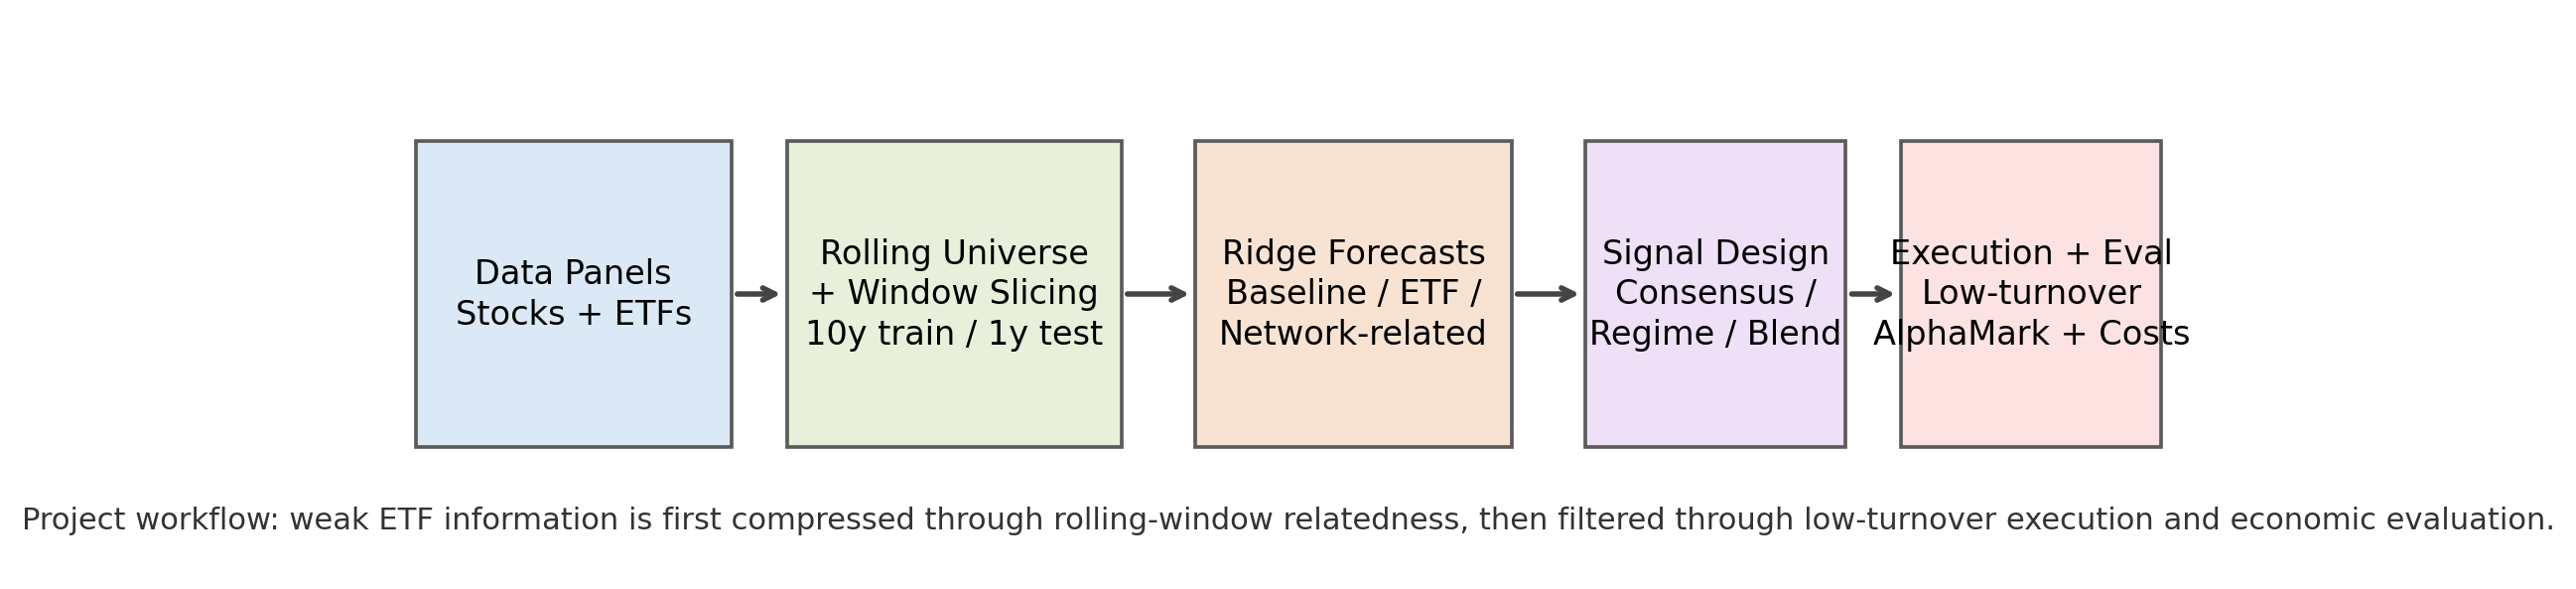
\includegraphics[width=\linewidth]{figures/pipeline_schematic.png}
\caption{Project workflow. ETF information is first summarized through rolling-window relatedness and then passed through explicit holding-period and rebalance rules before economic evaluation.}
\label{fig:pipeline}
\end{figure}

\subsection{Rolling-Universe Eligibility}

The stock universe is dynamic. For a stock to enter a given model in a given window, it must have the features and target required by that specific model inside the local train-test split. This detail matters because the eligible universe is not the same across the baseline, raw ETF, and network-style models. The resulting design is therefore both rolling in time and model-dependent in coverage.

\subsection{Ridge Regression and Feature Design}

All predictive models are estimated with Ridge regression. The initial model family includes:
\begin{itemize}[leftmargin=1.4em]
  \item a stock-only HAR baseline,
  \item a raw ETF model with a large ETF feature block,
  \item a network-style model using ETF-linked neighbor structure.
\end{itemize}

The stock-only HAR baseline has the form
\[
\hat r^{\mathrm{base}}_{i,t+1}
=
\beta_0+\beta_d r^{(d)}_{i,t}+\beta_w r^{(w)}_{i,t}+\beta_m r^{(m)}_{i,t}.
\]
The raw ETF model augments the baseline with a large set of daily ETF covariates available in the current window. The network-style model augments the baseline with a single neighbor-lag feature built from ETF-related stock similarity.

The raw ETF experiment is informative precisely because it fails: naive high-dimensional ETF expansion proves unstable and economically unconvincing. That result motivates the later stock-specific ETF summaries.

\subsection{Top-1 and Top-3 ETF Compression}

To reduce dimensionality, we summarize ETF information at the stock level through local relatedness. Let $\mathrm{Top1}(i)$ denote the ETF most related to stock $i$ within the current training window, and let $\mathrm{Top3}(i)$ denote the three most related ETFs. We then construct:
\[
\hat r^{\mathrm{top1}}_{i,t+1}
=
\hat r^{\mathrm{base}}_{i,t+1}
+ \gamma \, ETF^{\mathrm{Top1}(i)}_{d,t},
\]
\[
\hat r^{\mathrm{top3}}_{i,t+1}
=
\hat r^{\mathrm{base}}_{i,t+1}
+ \gamma \cdot \frac{1}{3}\sum_{e \in \mathrm{Top3}(i)} ETF_{e,d,t}.
\]

These ETF summaries are low-dimensional by construction and are much easier to interpret economically than a large raw ETF block.

\subsection{Network Feature Construction}

For the network-style models, we first construct a stock--ETF relatedness matrix inside the training window. This matrix is then converted into a stock--stock neighbor graph by comparing stocks through their ETF exposure patterns. For each stock, we keep the top-5 neighbors and define a lagged neighbor-return feature
\[
\mathrm{feat}^{\mathrm{nbr}}_{i,t}
=
\sum_{j \in \mathcal{N}_5(i)} w_{ij} r_{j,t},
\]
where the weights $w_{ij}$ are normalized across the selected neighbors. This feature is meant to capture peer effects implied by similarity in ETF linkage. In practice, however, the network-based specifications were not strong enough to become our final strategy family.

\subsection{Execution Layer}

Predicted signals are mapped to long-short portfolios. Let $s_{i,t}$ denote the selected strategy signal and let $\mathrm{bet\_size}_{i,t}$ denote either equal-weight sizing or lagged market-cap sizing. Daily portfolio weights are normalized as
\[
w_{i,t}
\propto
\mathrm{sign}(s_{i,t}) \cdot |\mathrm{bet\_size}_{i,t}|,
\qquad
\sum_i |w_{i,t}| = 1.
\]

The execution layer includes two turnover controls:
\begin{itemize}[leftmargin=1.4em]
  \item \texttt{hold\_days}: the minimum time before another rebalance is allowed;
  \item \texttt{rebalance\_threshold}: the minimum change between the current and target portfolios required to trigger a rebalance.
\end{itemize}

The target portfolio is only implemented if enough time has passed since the last rebalance and the desired portfolio differs sufficiently from the currently held one. This execution rule is central to the final results. Several signals that look attractive on a gross basis deteriorate quickly under costs when rebalanced too frequently, but remain viable under slower trading schedules.

\subsection{AlphaMark and Cost Sensitivity}

We use AlphaMark as the main standardized gross-performance evaluation tool. In the updated version of the project, AlphaMark is run with multiple quantile slices (\texttt{qr\_100}, \texttt{qr\_75}, \texttt{qr\_50}, and \texttt{qr\_25}) so that we can study whether the strongest performance appears in the full universe or in more selective parts of the signal ranking.

In addition, we run a separate tradability review under 10, 20, and 50 basis point cost assumptions. These basis-point costs should be interpreted as simplified all-in trading-cost scenarios that proxy for commissions, fees, spread, slippage, and market impact, applied proportionally to turnover:
\[
\mathrm{net\ return}_t
=
\mathrm{gross\ return}_t
-
\mathrm{turnover}_t \times c.
\]

This dual evaluation framework is deliberate. AlphaMark tells us whether the signal is economically meaningful on a gross basis, while the cost review tells us whether that apparent alpha survives a basic implementation test.

\section{Final Strategy Design}
\label{sec:strategy}

The final report focuses on three ETF-conditioned strategies. All three start from the same stock-only baseline, but they use ETF-linked information in different ways. They emerge from the same empirical pattern: direct ETF expansion and the pure network term do not deliver strong final strategies, whereas narrower ETF-based adjustments remain useful.

\subsection{Consensus Majority ETF}

This signal combines three forecasts: the baseline, the baseline plus the top-1 ETF daily term, and the baseline plus the top-3 ETF daily mean. A stock is traded only when at least two of the three forecasts agree on direction. In shorthand,
\[
s^{\mathrm{cons}}_{i,t}
=
\mathrm{MajorityVote}
\left(
s^{\mathrm{base}}_{i,t},
s^{\mathrm{top1}}_{i,t},
s^{\mathrm{top3}}_{i,t}
\right).
\]

Operationally, the signal is zero when there is no majority agreement, positive when at least two forecasts point up, and negative when at least two point down. The specification retained in the final evaluation uses lagged market-cap sizing, full-universe coverage ($q=1.0$), a 20-day minimum holding period, and a rebalance threshold of 0.3. The economic interpretation is that ETF information is most valuable when it corroborates, rather than overrides, the stock-only forecast.

\subsection{Regime Strategy}

We define a blended signal
\[
s^{\mathrm{blend}}_{i,t} = 0.7\, s^{\mathrm{base}}_{i,t} + 0.3\, s^{\mathrm{top3}}_{i,t}.
\]
When the market environment is strong, proxied by positive short-horizon SPY signals, we use the baseline. Outside that regime, we require agreement between the baseline and the ETF-conditioned top-3 signal; otherwise the trade is suppressed. In shorthand,
\[
s^{\mathrm{reg}}_{i,t}
=
\begin{cases}
s^{\mathrm{base}}_{i,t}, & \text{if the market regime is strong},\\
s^{\mathrm{blend}}_{i,t}, & \text{if the regime is weak and } \mathrm{sign}(s^{\mathrm{base}}_{i,t})=\mathrm{sign}(s^{\mathrm{top3}}_{i,t}),\\
0, & \text{otherwise.}
\end{cases}
\]
This makes ETF information contingent on market state rather than universally active. The most robust implementation uses equal weighting, full-universe coverage, a 20-day holding period, and a rebalance threshold of 0.1.

\subsection{Blend Top3}

This is the most conservative design. It simply uses the soft combination
\[
s^{\mathrm{blend}}_{i,t} = 0.7\, s^{\mathrm{base}}_{i,t} + 0.3\, s^{\mathrm{top3}}_{i,t}.
\]
The goal is not to let ETF information dominate, but to allow it to make a modest adjustment to the baseline. In the final cost-adjusted evaluation, the strongest stable version uses full-universe coverage and slower rebalancing, with the exact best sizing choice depending somewhat on the assumed cost level. Conceptually, this is the simplest specification: the stock-only signal remains primary, and ETF information tilts the ranking at the margin.

\subsection{Why These Three}

These strategies were selected because they remained competitive after exploratory screening, implementation constraints, AlphaMark evaluation, and transaction-cost sensitivity analysis. They also span three distinct uses of ETF-linked information:
\begin{itemize}[leftmargin=1.4em]
  \item \textbf{confirmation}: consensus majority ETF,
  \item \textbf{conditioning}: regime strategy,
  \item \textbf{correction}: blend top3.
\end{itemize}

Together they support a common interpretation: ETF-linked information is not strong enough to drive the model on its own, but it can improve the baseline when introduced in a narrower and more disciplined form.

\section{Results}
\label{sec:results}

\subsection{From Negative $R^2$ to Economic Evaluation}

The early model comparison gave a clear warning sign: raw ETF expansion was not a robust way to improve daily stock-return prediction. Out-of-sample $R^2$ was generally negative, and the raw ETF model underperformed due to dimensionality and noise. This negative result is important because it motivates the later design choice: compress ETF information and evaluate it economically rather than relying on statistical fit alone.

\subsection{Initial Four-Model Comparison}

The first clean lesson comes from the initial four-model comparison: baseline, baseline+ETF, baseline+network, and baseline+ETF+network. Table~\ref{tab:initial-models} reports the gross AlphaMark Sharpe ratios at the full-universe slice (\texttt{qr\_100}).

\begin{table}[H]
\centering
\caption{Initial four-model comparison using gross AlphaMark Sharpe at \texttt{qr\_100}.}
\label{tab:initial-models}
\begin{tabular}{lcc}
\toprule
Model & cap250k & mktcap \\
\midrule
Baseline HAR & 0.604 & 0.657 \\
Baseline + raw ETF block & 0.311 & 0.099 \\
Baseline + network & -0.094 & -0.052 \\
Baseline + ETF + network & 0.087 & -0.020 \\
\bottomrule
\end{tabular}
\end{table}

This table and Figure~\ref{fig:initial-models} capture the central empirical tension in the project. The baseline is strong. The raw ETF block does not improve on it and often performs much worse. The network-style extension is conceptually interesting, but in this implementation it does not survive as a competitive gross strategy. These early results indicate that the incremental content in ETF-linked variables is limited when used directly and requires a narrower specification.

\begin{figure}[H]
\centering
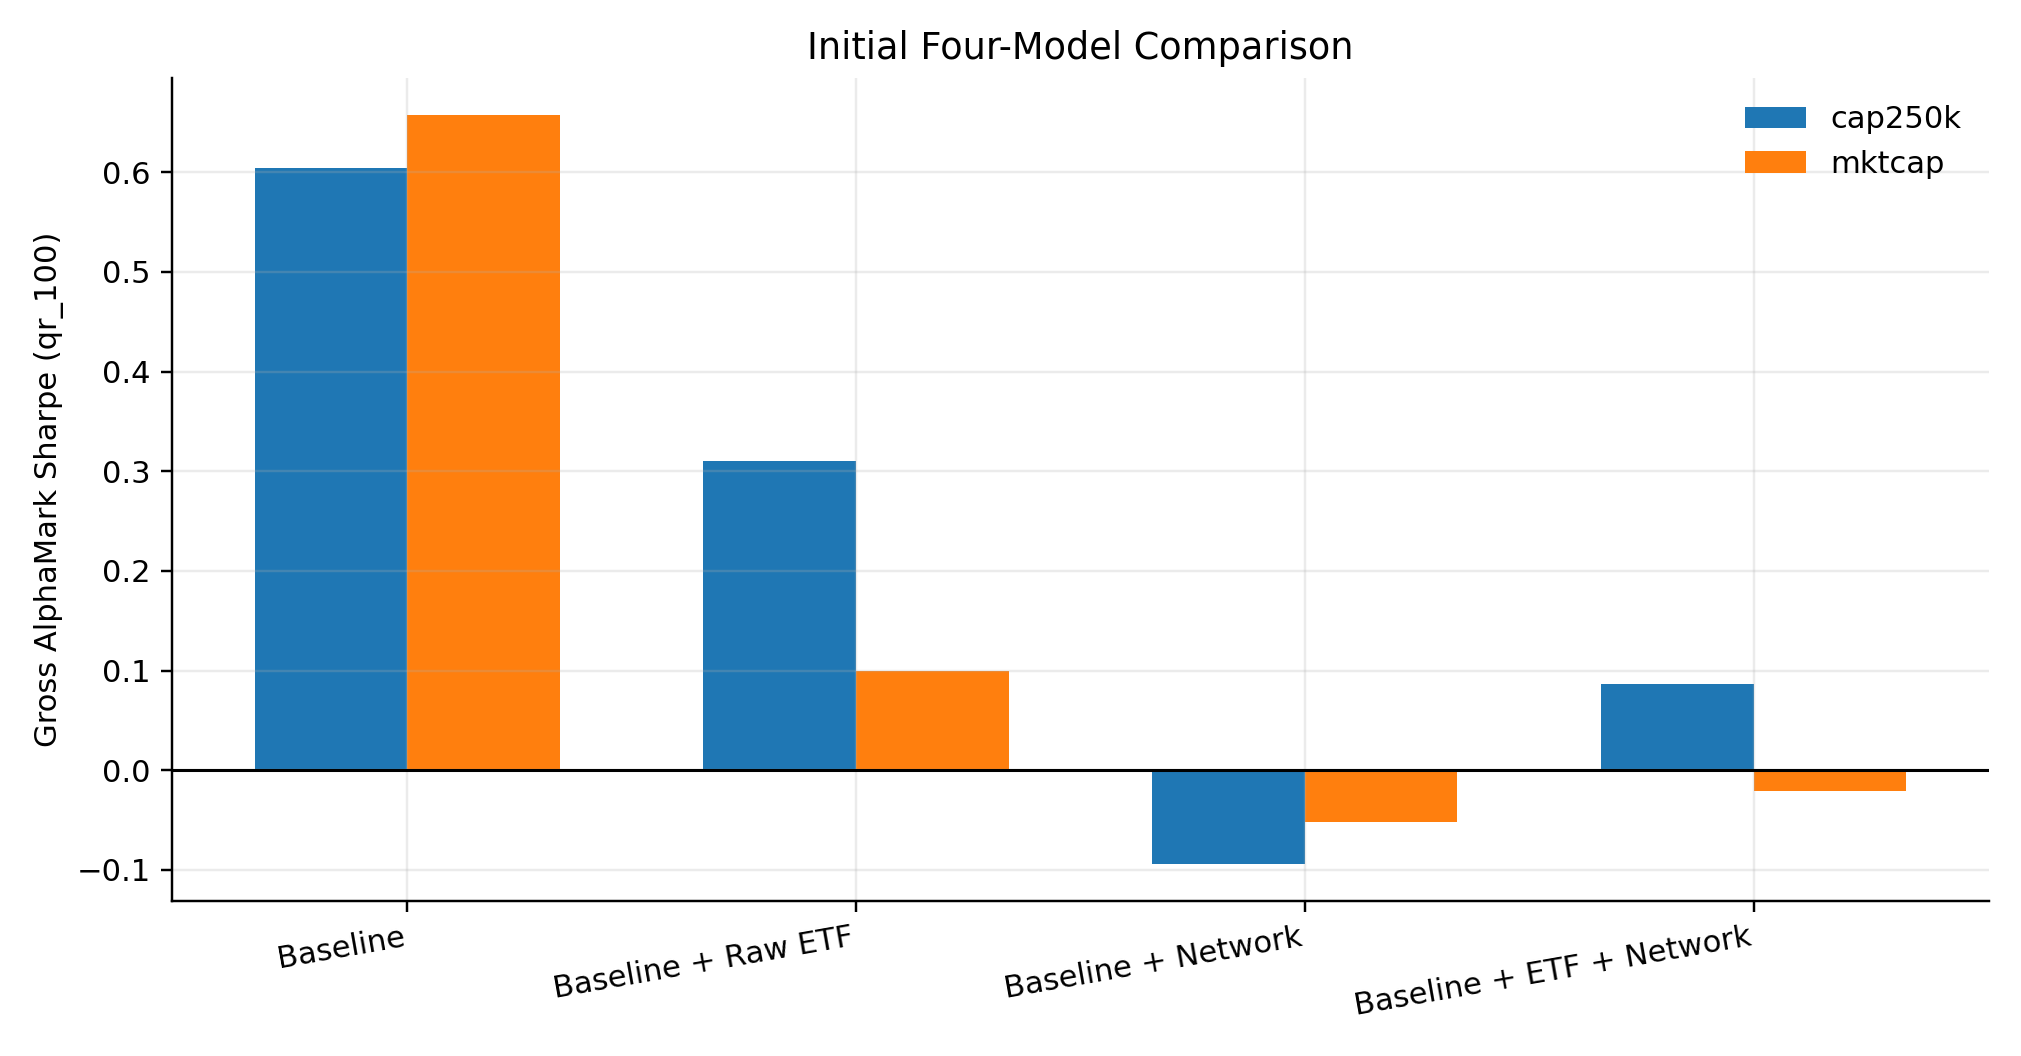
\includegraphics[width=0.92\linewidth]{figures/initial_model_comparison.png}
\caption{Gross AlphaMark Sharpe for the initial four-model comparison at \texttt{qr\_100}. The main empirical message is that the stock-only baseline is strong, raw ETF expansion is much weaker, and the pure network-style extension does not become competitive in this implementation.}
\label{fig:initial-models}
\end{figure}

\subsection{Cost-Adjusted Ranking of Final Strategies}

Table~\ref{tab:final-strategies} summarizes the three final strategies. The strongest 20 bps net result is the consensus-majority ETF strategy, while the regime strategy is the most resilient at higher cost levels. The baseline remains a strong benchmark once it is evaluated under comparable execution constraints, so the appropriate interpretation is not ``ETF beats baseline everywhere.'' Rather, ETF-conditioned strategies become competitive and in some settings superior once the trading rule is specified carefully.

\begin{table}[H]
\centering
\caption{Summary of the final low-turnover strategies. Gross AlphaMark Sharpe is shown using the strongest quantile slice from the updated multi-quantile AlphaMark reports. Net Sharpe numbers come from the separate turnover-based cost review.}
\label{tab:final-strategies}
\begin{tabular}{lcccc}
\toprule
Strategy & Best gross Sharpe & Net 10 bps & Net 20 bps & Net 50 bps \\
\midrule
Consensus majority ETF & 0.558 & 0.482 & 0.417 & 0.221 \\
Blend top3 & 0.598 & 0.419 & 0.373 & 0.259 \\
Regime & 0.525 & 0.452 & 0.404 & 0.279 \\
Optimized baseline benchmark & 0.657 & 0.500 & 0.373 & 0.259 \\
\bottomrule
\end{tabular}
\end{table}

The ranking across cost regimes is informative, as summarized in Figure~\ref{fig:cost-robustness}. At 10 bps, the optimized baseline remains extremely strong. At 20 bps, the consensus-majority ETF strategy becomes the strongest of the final three and slightly exceeds the optimized baseline benchmark. At 50 bps, the regime strategy becomes relatively more robust. This pattern is consistent with ETF-linked information being most useful when it helps screen marginal trades rather than when it is used to support frequent repositioning.

Appendix~\ref{sec:appendix-impl} records the exact rolling-window design and the representative implementation parameters used in the central 20 bps comparison.

\begin{figure}[H]
\centering
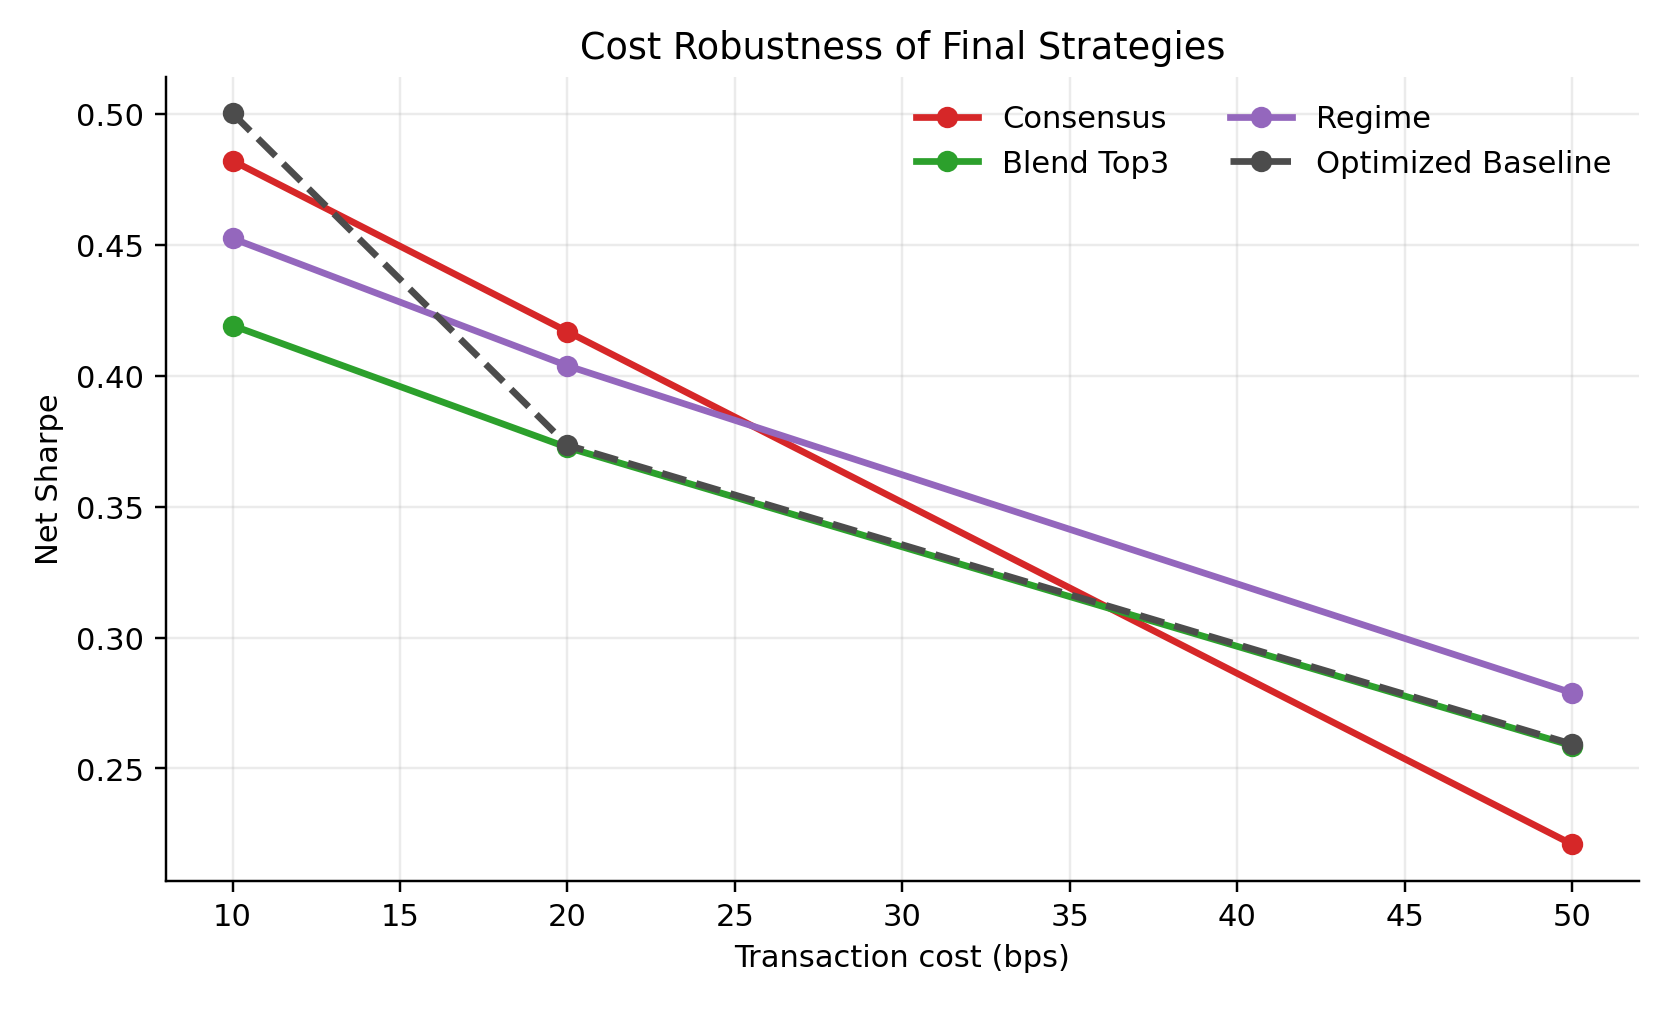
\includegraphics[width=0.84\linewidth]{figures/cost_robustness.png}
\caption{Net Sharpe under 10, 20, and 50 bps cost assumptions. The optimized baseline remains a strong benchmark, but the ETF-conditioned strategies become competitive once execution is slowed down, with consensus strongest around 20 bps and regime most resilient at 50 bps.}
\label{fig:cost-robustness}
\end{figure}

Figure~\ref{fig:net-paths} plots the cumulative net return paths for the central 20 bps case. This is the cleanest like-for-like comparison because it uses each strategy's representative implementation under the same cost assumption. The figure shows that the ETF-conditioned strategies are not merely producing isolated high-Sharpe summaries; they also generate sustained cumulative performance paths that are comparable to, and in some periods stronger than, the optimized baseline.

\begin{figure}[H]
\centering
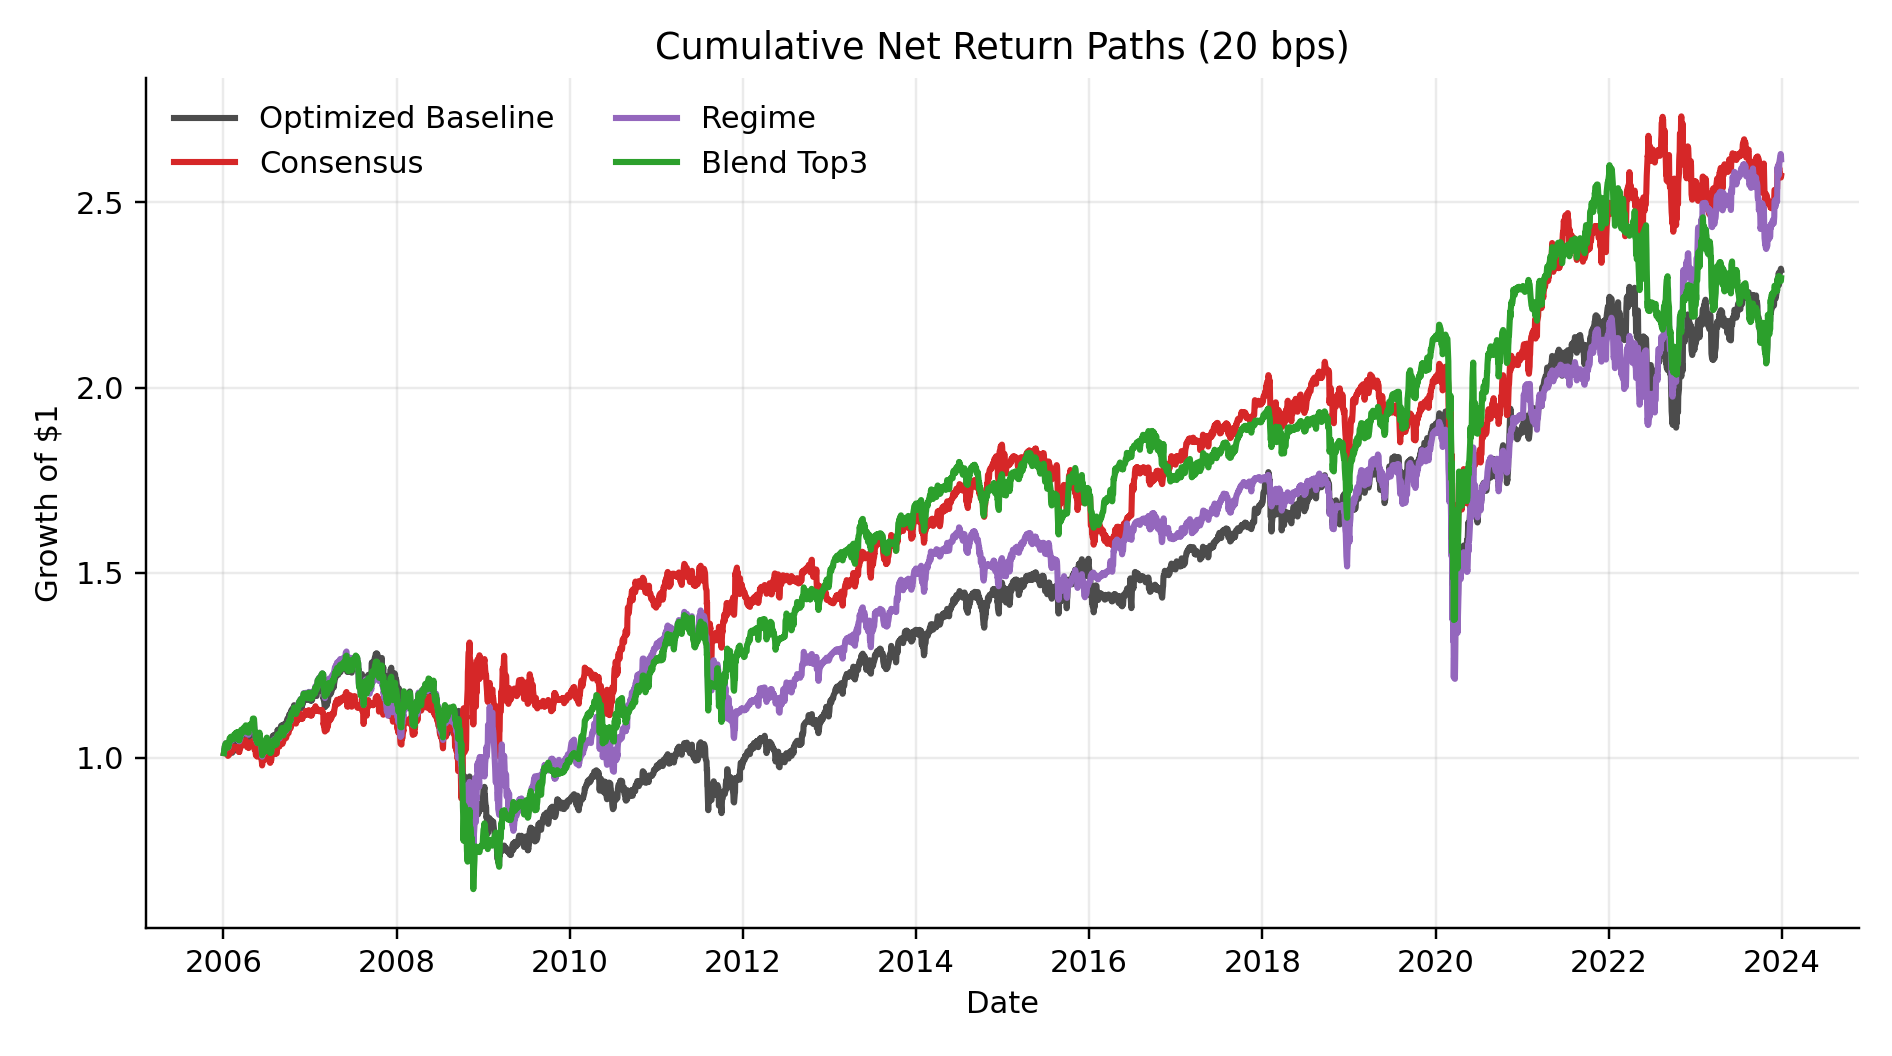
\includegraphics[width=0.88\linewidth]{figures/net_cumulative_paths_20bps.png}
\caption{Cumulative net return paths at 20 bps for the optimized low-turnover baseline and the three final ETF-conditioned strategies. This central-cost comparison makes the economic significance of the strategies visually transparent and highlights that the final strategies should be viewed as competitive refinements to a strong baseline benchmark.}
\label{fig:net-paths}
\end{figure}

\subsection{AlphaMark Quantile Results}

The updated AlphaMark reports now include \texttt{qr\_100}, \texttt{qr\_75}, \texttt{qr\_50}, and \texttt{qr\_25}. This matters because the best slices do not always occur at the full-universe level. For example, the strongest gross AlphaMark Sharpe for the consensus strategy occurs at \texttt{qr\_75} with market-cap sizing (about 0.558), while the strongest gross slice for the blend and regime strategies appears around \texttt{qr\_50} with equal-weight sizing (about 0.598 and 0.525, respectively).

This quantile evidence, visualized in Figure~\ref{fig:qmulti}, supports the general interpretation that the signals contain useful cross-sectional ranking information even when the full-universe portfolio is not always the best-performing gross configuration. Put differently, ETF-conditioned signals do not merely alter average portfolio exposure; they also help reshape the cross-sectional ordering of names.

\begin{figure}[H]
\centering
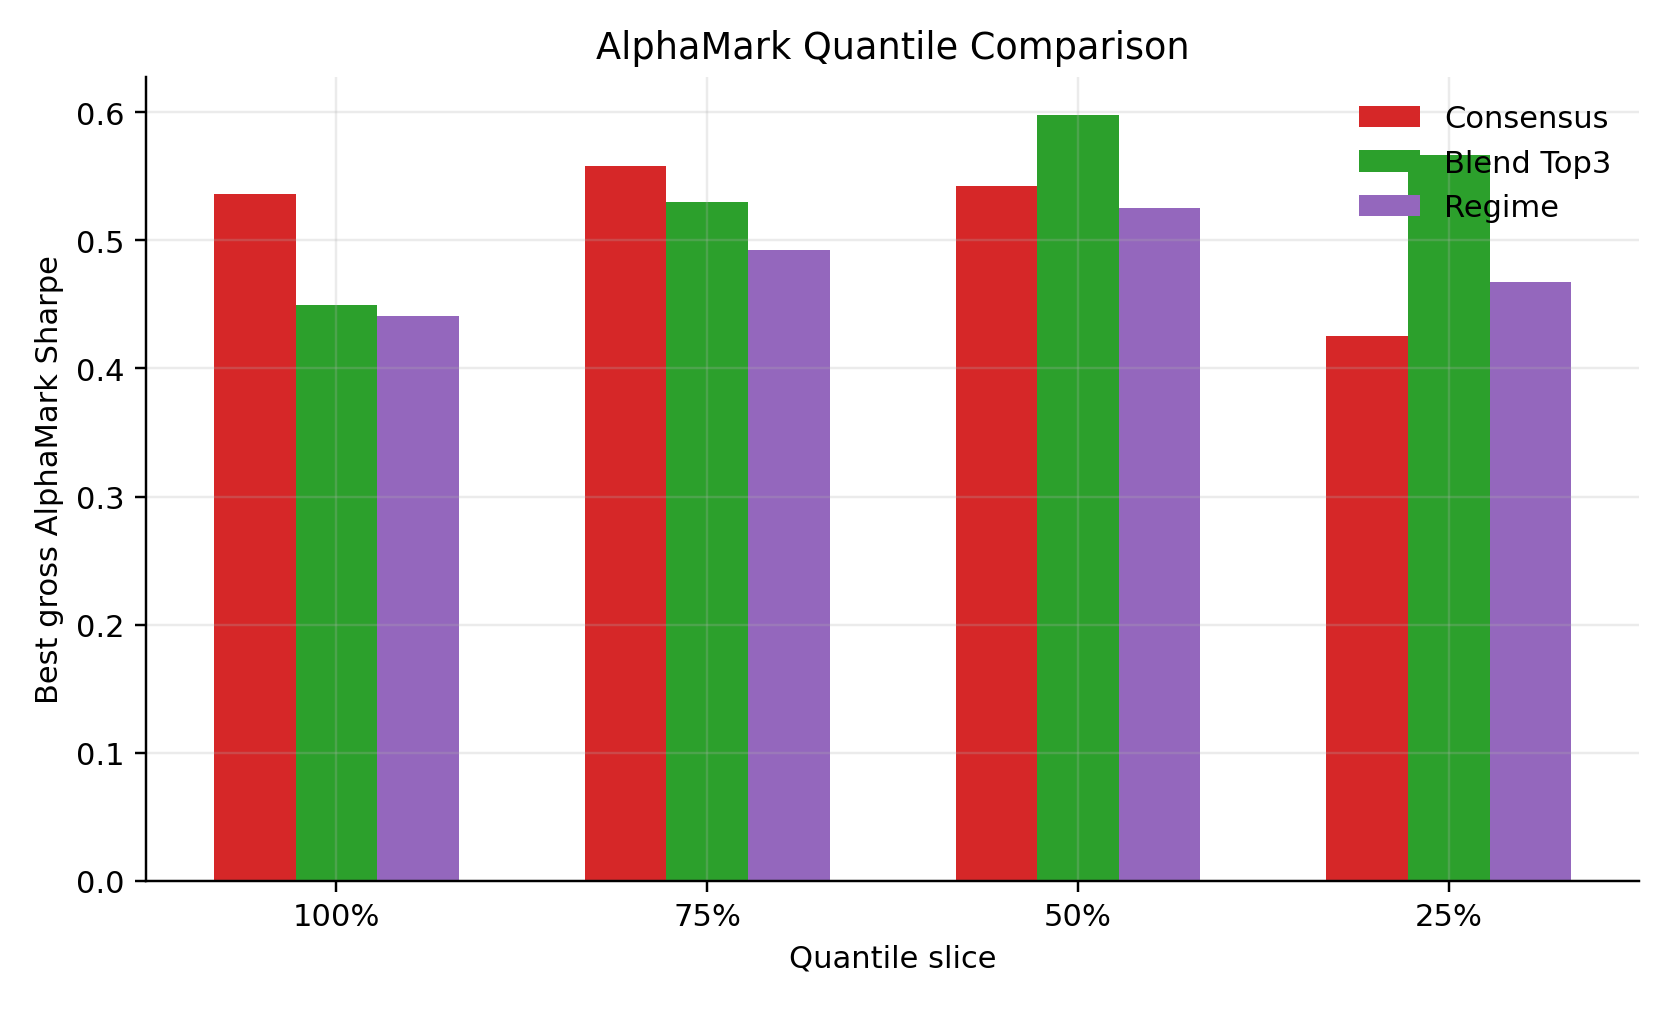
\includegraphics[width=0.84\linewidth]{figures/alphamark_quantile_comparison.png}
\caption{Best gross AlphaMark Sharpe by quantile slice for the three final strategies. The strongest slice is not always the full-universe portfolio, which suggests that the ETF-conditioned signals contain useful cross-sectional ranking information.}
\label{fig:qmulti}
\end{figure}

\subsection{Liquidity Diagnostic}

We also ran a normalized-dollar-volume bucket analysis. The main result is not that one specific liquidity bucket drives all performance. In fact, when the strategy is restricted to a single bucket, net Sharpe typically worsens. However, on a gross basis, the ETF-conditioned strategies look cleaner in the middle-to-upper liquidity buckets than in the extreme low- or high-activity buckets. For instance, the consensus strategy is strongest in the middle buckets on a gross basis, whereas single-bucket net performance remains poor across the board.

This suggests that ETF-linked information may be more reliable in moderate liquidity states, but that the final alpha still needs broad cross-sectional diversification to survive costs. In other words, normalized liquidity is a useful diagnostic variable, but not a sufficient standalone trading filter. Figure~\ref{fig:liquidity} is therefore best read as an implementation diagnostic rather than as an argument for a single-bucket trading rule.

\begin{figure}[H]
\centering
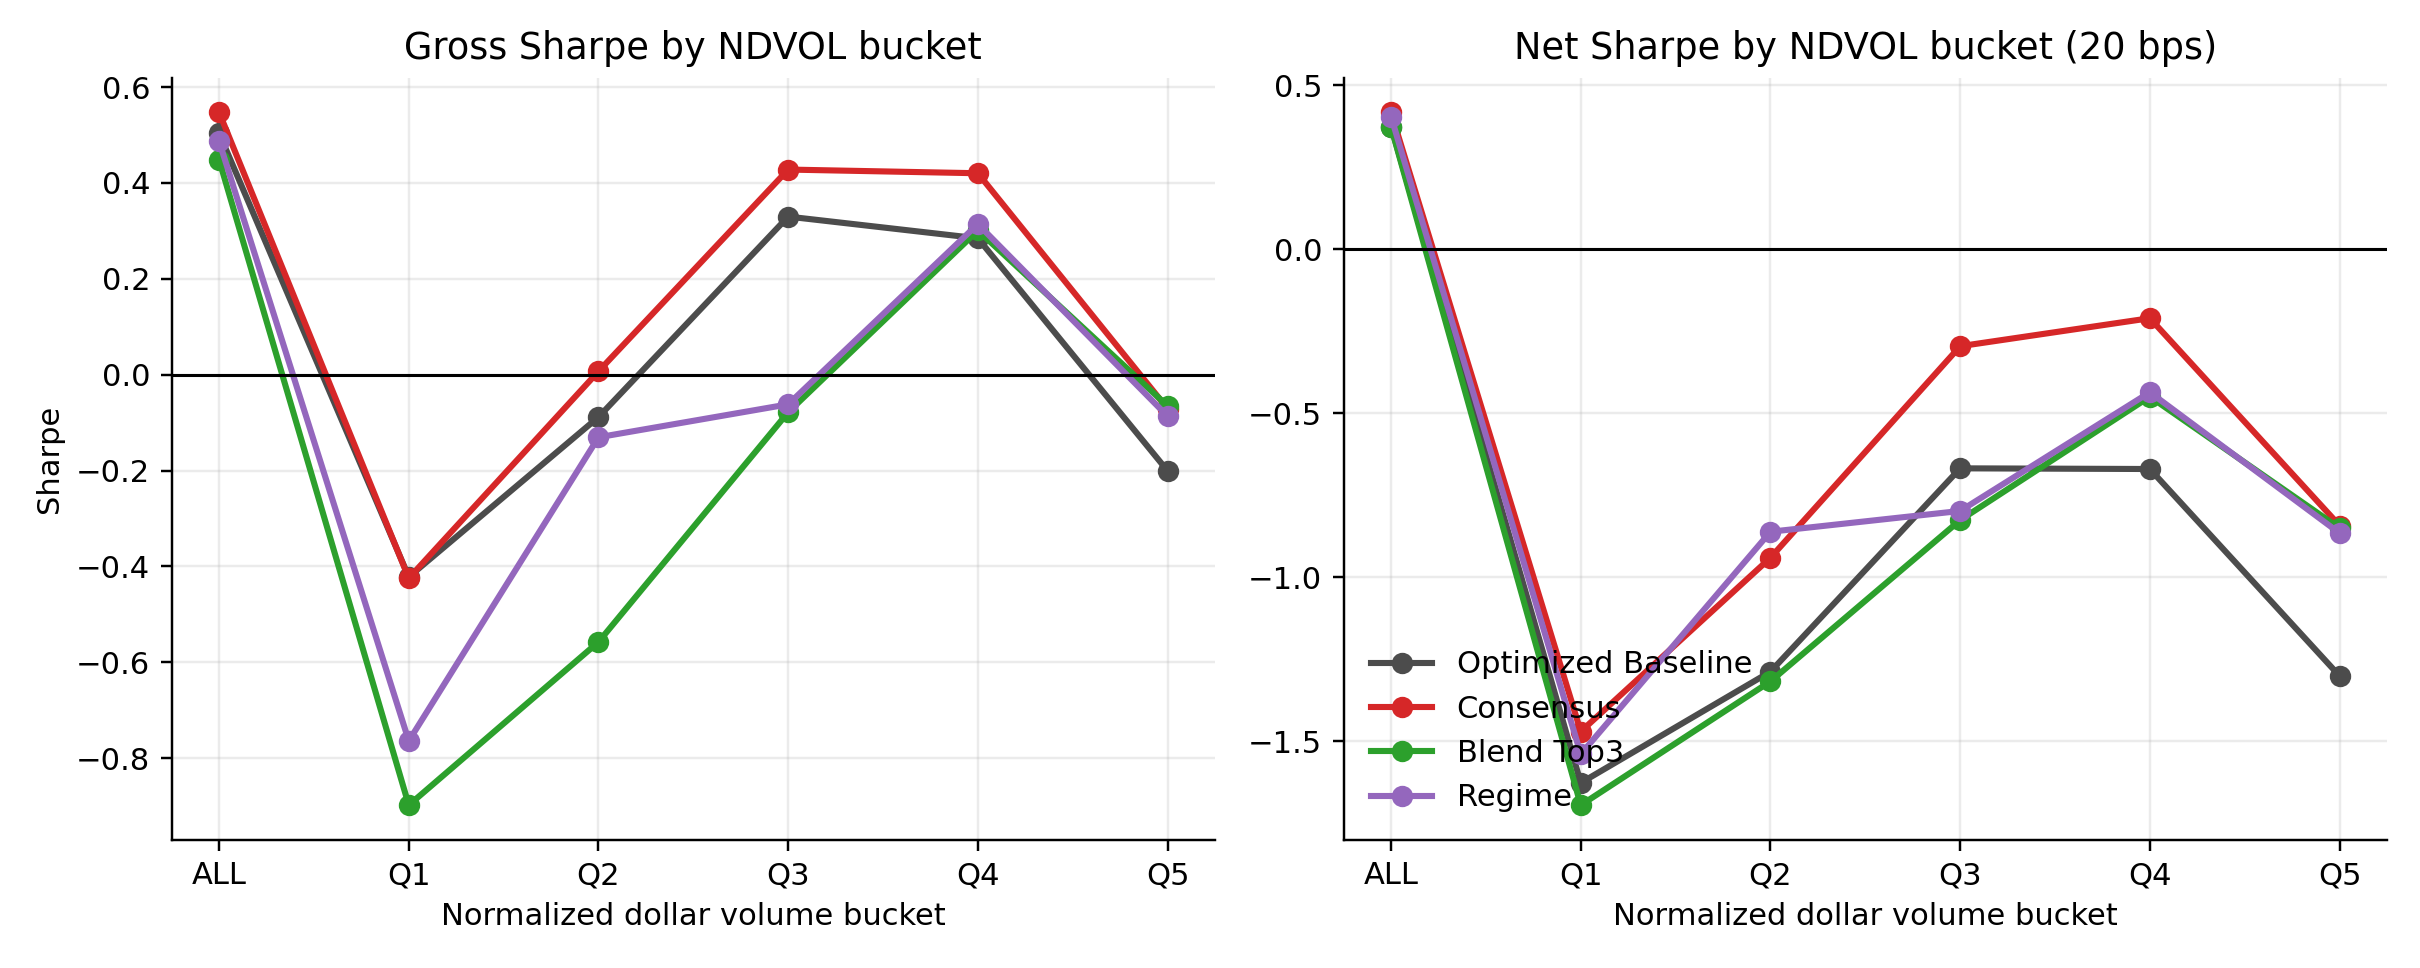
\includegraphics[width=\linewidth]{figures/liquidity_bucket_diagnostic.png}
\caption{Liquidity-state diagnostic based on normalized dollar volume (NDVOL). On a gross basis, the ETF-conditioned strategies look cleaner in the middle buckets. On a net basis, restricting the strategy to a single bucket worsens performance, which suggests that broad cross-sectional diversification remains important.}
\label{fig:liquidity}
\end{figure}

\section{Discussion}
\label{sec:discussion}

\subsection{Interpretation}

The evidence does not support the claim that ETF information is a strong standalone forecasting signal. The stock's own HAR history remains the dominant source of predictive content. At the same time, the results do not justify treating ETF information as irrelevant. It adds value most clearly when it is used to validate, adjust, or selectively suppress the stock-only signal.

The most defensible interpretation is that ETF-linked information has limited incremental content when entered directly, but remains useful when introduced through narrower and more disciplined specifications. Raw ETF expansion performs poorly, whereas Top-1 / Top-3 summaries and related filtering rules improve economic performance. The appropriate conclusion is therefore not ``ETF beats the baseline,'' but ``ETF can refine the baseline under a more selective design.'' The correct comparison is against a baseline that is itself given a reasonable implementation rule, and under that benchmark the ETF-conditioned strategies are best described as competitive, interpretable refinements.

\subsection{Methodological Novelty}

The novelty of the project is not a single new estimator. Instead, it lies in the combination of design choices:
\begin{itemize}[leftmargin=1.4em]
  \item a rolling-universe window-slicing setup rather than a fixed long-horizon panel,
  \item the shift from statistical significance to economic significance,
  \item the use of ETF-linked information as conditional information rather than as a raw feature block,
  \item the explicit turnover-aware execution layer,
  \item and the liquidity-state diagnostic based on normalized dollar volume.
\end{itemize}

In that sense, the project adds something beyond a standard forecasting exercise: the contribution lies in how ETF-linked information is represented, filtered, and translated into a tradable signal.

\subsection{Relation to the Original Network Idea}

It is also important to be transparent about the network component. The original project motivation was strongly connected to peer effects and ETF-based network structure. That idea remains conceptually useful and informed the way we think about ETF-linked similarity. However, the pure network-style model did not emerge as the strongest final implementation. That should be presented as a substantive empirical finding: the network intuition helped motivate the exploration, but the strongest economic results came from narrower ETF-conditioned adjustments rather than from the network term alone.

\subsection{Limitations}

Several limitations remain. First, the network formulation did not emerge as the strongest final strategy, even though it was part of the original motivation. Second, the cost model is deliberately simple and should be interpreted as a stress-test device rather than a full execution simulator. Third, the final report should be careful not to overclaim generality from a specific U.S. equities sample and a specific ETF feature universe.

These limitations do not invalidate the project, but they should shape the tone of the final write-up. The right claim is that ETF-linked information can become economically useful under a more selective representation and explicit execution controls, not that it universally dominates simpler baselines. Framed this way, the report contributes a disciplined empirical answer to a narrower and more realistic question: how should cross-asset information be organized so that it has a chance to survive implementation?

\section{Conclusion}

This project began with a simple idea: augment stock-level daily return prediction with ETF-linked information. The first pass showed that this idea does not work well in a naive form. Large raw ETF feature blocks perform poorly, and statistical forecasting metrics alone do not capture whether the resulting signals are economically useful.

The final outcome is more nuanced. ETF-linked information does not replace the stock-only HAR baseline, and it does not uniformly dominate an optimized baseline benchmark. What it can do is refine that benchmark. Once the information is summarized through stock-specific signals and combined with rolling-universe training, explicit execution rules, and PnL-based evaluation, it becomes economically meaningful. In this sense, the project's contribution is less about discovering a strong new standalone predictor and more about showing how cross-asset information can be organized into a tradable signal.

Among the final strategies, consensus-majority ETF, regime-dependent refinement, and blend top3 each capture a different way in which ETF-linked information can improve the baseline. Taken together, they support a broader conclusion: in noisy financial prediction settings, the main challenge is not only learning a signal, but also deciding how to represent it, when to trust it, and how to trade it. This is why the report emphasizes methodology, economic evaluation, and execution discipline alongside predictive modeling.


\appendix
\section{Implementation Notes and Reproducibility}
\label{sec:appendix-impl}

\subsection{Rolling Window Schedule}

The final evaluation period is 2006--2023. We use 18 annual test slices, each paired with a 10-year training window. For a test year $Y$, the training sample uses the preceding ten calendar years. For example, the first reported slice trains on 1996--2005 and tests on 2006, while the final slice trains on 2013--2022 and tests on 2023. All model components are re-estimated separately in each slice, including stock--ETF relatedness, Top-1 / Top-3 ETF selection, and any network-style neighbor structure.

\subsection{AlphaMark and Cost Settings}

The updated AlphaMark runs use four quantile slices:
\[
\texttt{qr\_100},\quad
\texttt{qr\_75},\quad
\texttt{qr\_50},\quad
\texttt{qr\_25},
\]
and the standard sizing conventions \texttt{betsize\_cap250k} and \texttt{betsize\_mktcap\_lag}. These AlphaMark outputs are interpreted as gross performance diagnostics.

Separately, we run a turnover-based tradability review at 10, 20, and 50 basis points. Throughout the report, 20 bps is the central cost case because it is conservative enough to be meaningful while still allowing differences across strategies to remain visible.

\subsection{Representative Low-Turnover Hyperparameters}

Table~\ref{tab:appendix-centralcase} records the representative low-turnover settings for the central 20 bps case. These are the configurations used when comparing the final three ETF-conditioned strategies against the optimized baseline benchmark on a net basis.

\begin{table}[h]
\centering
\caption{Representative low-turnover settings for the central 20 bps comparison.}
\label{tab:appendix-centralcase}
\begin{tabular}{lccccc}
\toprule
Strategy & Bet size & $q$ & Hold days & Threshold & Net 20 bps Sharpe \\
\midrule
Optimized baseline & mktcap lag & 1.0 & 10 & 0.2 & 0.373 \\
Consensus majority ETF & mktcap lag & 1.0 & 20 & 0.3 & 0.417 \\
Regime & equal & 1.0 & 20 & 0.1 & 0.404 \\
Blend top3 & equal & 1.0 & 20 & 0.1 & 0.373 \\
\bottomrule
\end{tabular}
\end{table}

\subsection{Best Gross Quantile Slices}

The strongest gross AlphaMark slices differ across strategies. The consensus strategy is strongest at \texttt{qr\_75} with market-cap sizing (gross Sharpe about 0.558), while the blend and regime strategies are strongest around \texttt{qr\_50} with equal-weight or cap250k-style sizing (gross Sharpe about 0.598 and 0.525, respectively). This is why the main text reports both gross AlphaMark outcomes and separate net-of-cost results: the gross-optimal slice is not always the net-optimal execution policy.


\bibliographystyle{plainnat}
\bibliography{references}

\end{document}
